% !TeX root = ../main-paper.tex
\section{Experimental Setup}


\begin{figure}[tb]
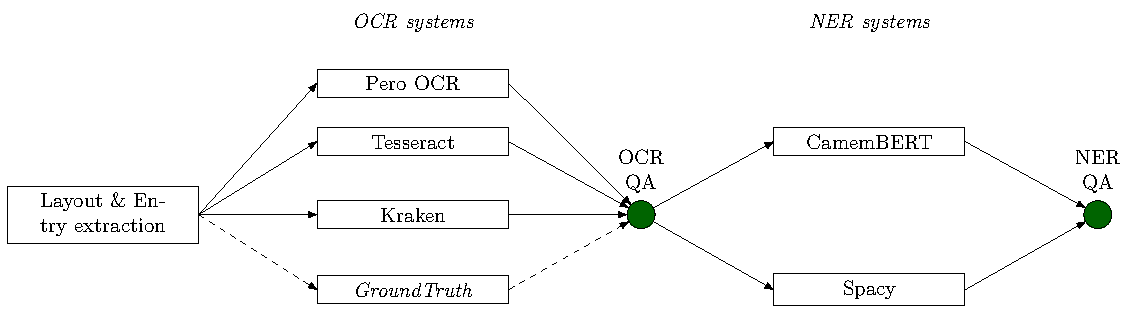
\includegraphics[width=\linewidth]{figs/protocol.pdf}
\caption{Scheme of the evaluation protocol. \joseph{Missing "Ground truth" for NER stage?}}
\label{fig.protocol}
\end{figure}

\subsection{Evaluation protocol \& Metrics}

The Figure \Cref{fig.protocol} depicts the evaluation protocol used to assess the OCR and NER systems. Two quality evaluations
are performed in the pipeline, respectively named \emph{OCR Q.A.} and \emph{NER Q.A.}.

First, the layout extraction and entry segmentation of the page are performed with a semi-automated system and
checked by a human. Afterward, an OCR system runs on the thumbnails of each segmented entry to extract its text. An
entry might span over multiple text lines but is always a single block. Thus, the most adapted mode is chosen when
the OCR system allows for the detection mode (e.g. the \emph{block} mode for \emph{Tesseract}). 

\textbf{OCR Q.A.} is performed after some text normalization of the OCR system outputs. Text normalization consists in
projecting Unicode characters onto the latin-1 charset (whenever it makes sense) and removing extra symbols (hands,
crosses). Then, the predicted text is aligned with the reference text using standard tools and the Character Error Rates
(CER) are computed at the entry level and at the global level. 

\begin{align}
\mathrm{CER} &=  \frac{\#Errors}{\text{Reference Text Length}} & & \mathrm{CER}_\mathrm{norm} =  \frac{\#Errors}{\text{Alignment Length}} 
\end{align}

In this benchmark, we consider 3 OCR systems well known for historical document analysis: Pero OCR, Tesseract, and Kraken. 

\edwin{FIXME: add ref papier eval OCR + ISRI, eval KRAKEN}


Next, a NER system extracts the named entities from the text of each entry output by the OCR and the \textbf{NER Q.A.}
is performed. The NER system outputs a text with tags that enclose the entities. To assess the quality of the entity
extraction, we rely on a technique similar as for the OCR evaluation. The predicted text is aligned with the reference
text and the tags are projected in the alignment. Then, the precision, recall, and f-measure (or f-score) are computed considering
only the exact matches between entities. Precision and recall are defined by equation (2); the f-measure is their harmonic mean.

\begin{align}
    \mathrm{precision} &= \frac{\text{\#exact matches}}{\text{\#entries in prediction}} & \mathrm{recall} &= \frac{\text{\#exact matches}}{\text{\#entries in reference}}
\end{align}


The whole process is illustrated on~\cref{fig.eval-ocr-ner}. The OCR text and the GOLD text are first aligned to
evaluate the OCR accuracy. As there are 11 mismatches over 56 aligned characters, the CER is thus 24\%. This alignment
is then used to back-project the GOLD tags to build the tagged NER reference string. Finally, the NER system runs on the
OCR text; its output is compared to the NER reference string. There is only 2 over 3 tags matching in the prediction (precision),
while only 2 over 4 entities are matched in the reference (recall). It follows an overall f-score of 0.4.

\begin{figure}[tb]
    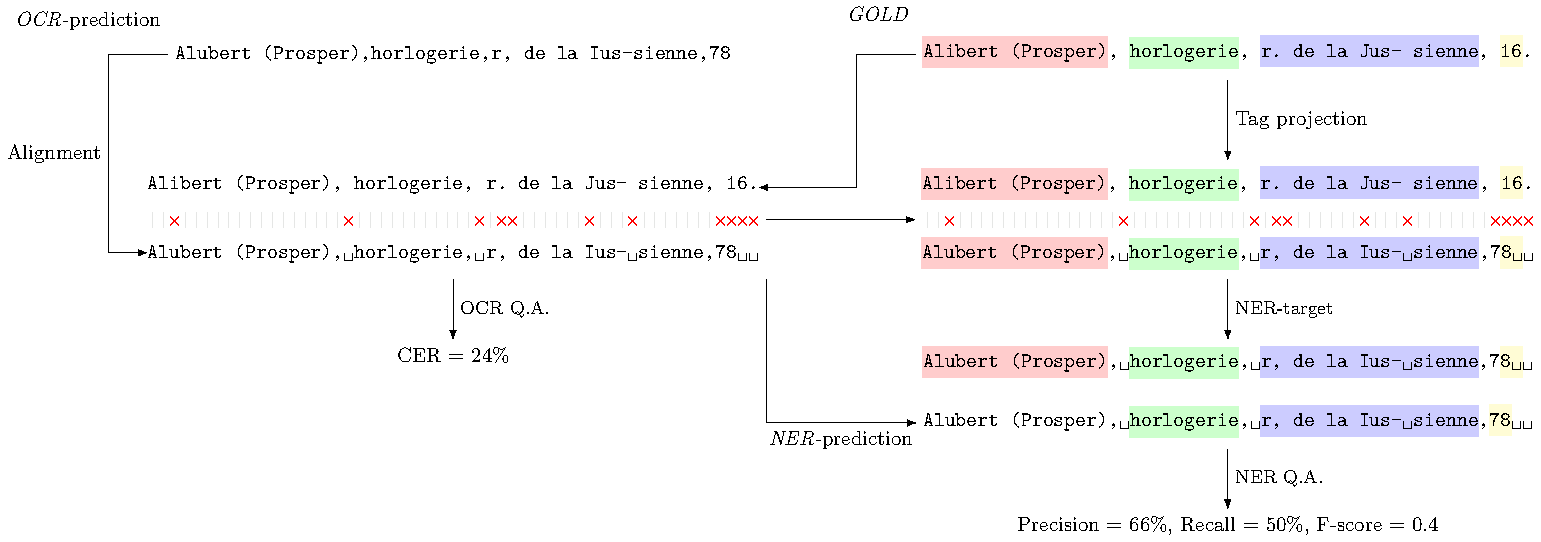
\includegraphics[width=\linewidth]{figs/eval-ocr-ner.pdf}
    \label{fig.eval-ocr-ner}
    \caption{OCR and NER evaluation protocol example.}
\end{figure}


\subsection{Experiment 1: NER sensibility to the number of training examples}
\label{subsection:experiment-1-setup}
\bertrand{Find a better name ?}
The constitution of annotated example sets to train a NER model on a target domain a is a critical preliminary step.
Often done manually, possibly from bootstrapped annotations, this task is tedious, time consuming and error prone.
The ability of a model to perform well even with few training examples is a pratical criteria to consider.
In this first experiment, we investigate the performance of the three models when fine-tuned for NER on training sets of decreasing sizes.

To do so, we split the gold reference of manually annotated entries into a training set, a development set, and a test set. 
The training set is then gradually reduced in size while maintaining the relative frequency of directories within it.

As the organisation and structure of entries varies across directories, the models may learn to overfit on a subset of directories with specific features.
To reduce the evaluation bias, we start by leaving out 3 directories (1690 entries, $\approx 19\%$) from the gold reference to test each model on unseen directories.
Then, a stratified sampling based on the source directory of each entry is run on the remaining set to create a training (6373 entries, $\approx 73\%$ of the gold reference) and a development set (709 entries, $\approx 8\%$).
This sampling procedure is a convenient way to shape both sets so they reflect the diversity of directories within the gold reference.
The development set is used to evaluate the models performance during the training phase.
To generate smaller training sets, we start from the initial training set and iteratively split it in half using the same stratified sampling strategy as before.
We stop if a directory has only one entry left, or if the current training subset contains less than 30 entries.
Applying this procedure to the initial training set produced 8 training subsets containing 49, 99, 199, 398, 796, 1593, 3186, and 6373 entries.

All tree models are fine-tuned for NER on each training subset.
The performance metrics are measured against the test set after each training.


% Move to results
%All metrics are evaluated on the test set, yet the biased metrics on the development set are added in the article material as additional information.


\subsection{Experiment 2: Impact of OCR nosie on named entity recognition}
\label{subsection:experiment-2-setup}
\bertrand{Assume that we use Kraken too. If not, adapt in consequence.}
Noise introduced by OCR is known to impede the named entity recognition process (see section~\ref{subsection:stoa-ner-on-historical-texts}).
%The second experiment assesses the impact of the OCR on the quality of the NER results.
The second experiment addresses two questions (1) which model is the most robust to OCR noise and (2) what is the most appropriate strategy to fine-tune the NER layer if the input texts to label are noisy ?
To this end, we leverage the labeled OCR datasets produced following to the method explained in Section 5, in addition to the gold reference.

First and foremost, to make sure that the datasets contain the same entries a preprocessing step must be performed.
Indeed, entries where the OCR produced an empty string and those for which no entity could be projected from the gold reference text are ignored.
To overcome this problem we filter each dataset by keeping only the entries common to all.
At the cost of losing  5\% of the gold references entries, we thus have four new annotated datasets containing the exact same entries.
They are denoted hereafter {reference, pero, tesseract, kraken}-gold.
Finally each is is split into a training, a dev and a test subset following the procedure presented in\cref{subsection:experiment-1-setup}.

We fine-tune CmBERT and CmBERT+ptrn on reference-gold and pero-gold to create two versions of each model: the former trained on manually corrected entries and the latter on OCR entries.
SpaCy NER is left aside as results from experiment 1 show that it is outperformed by BERT models.
Performance metrics are computed for each of the four resulting NER models against the test sets created from reference-gold, pero-gold, tesseract-gold and kraken-gold.

\subsection{Implementation details}

\subsubsection{OCR system parameters}
\nathalie{Y a-t-il des précisions à ajouter sur la façon dont ont été utilisés les OCR? Ou bien ce sont les versions "sur étagère" qui ont servi?}
\joseph{Totalement sur l'étagère. On a normalisé un peu les données après, c'est tout.}
\begin{itemize}
    \item Tesseract 4.1.1 (newest version: 5, released Nov. 2021)
    \item Pero OCR version from git repo, master branch updated on Sep 15, 2021 % 8b20f29    
    \item other?  % kraken if times allows
\end{itemize}

Pero OCR uses ParseNet \joseph{TODO ref} as internal layout parser for line detection.
Pero OCR uses an LSTM engine \joseph{TODO check + ref} for text line recognition.
Pero OCR generally works very well, as long as the bounding boxes of the regions to recognize are not too tightly adjusted.
Trained on newspapers in European languages by its development team.
Can output results in Latin, Greek and Cyrillic scripts, as well as some commonly-used typographic symbols.

% PERO refs
% O Kodym, M Hradiš: Page Layout Analysis System for Unconstrained Historic Documents. ICDAR, 2021.
% M Kišš, K Beneš, M Hradiš: AT-ST: Self-Training Adaptation Strategy for OCR in Domains with Limited Transcriptions. ICDAR, 2021.
% J Kohút, M Hradiš: TS-Net: OCR Trained to Switch Between Text Transcription Styles. ICDAR, 2021.


\subsubsection{Spacy}
We use the French model \textit{fr\_core\_news\_lg} provided by Spacy\mcite{spacy} library and leverage the library utilities to fine-tune it on various training and validation datasets derived from our ground truth dataset (see Section 5.2 for details). The base model is fine-tuned in turn on each of the 8 generated training datasets, using the same training parameters. Early stopping is activated with patience parameters set at 1600. For each size of the training dataset, 5 runs are performed, always with the same parameters, and the mean value of each performance score is computed.

%and Huggingface for the BERT 
%tok2vec(words embeddings + encoding) + attention layer  +  transition-based %model.

\subsubsection{Huggingface CamemBERT}
We start from the CamemBERT-ner model already fine-tuned on WikiNER-fr corpus and published on the Hugging Face repository \footnote{\url{https://huggingface.co/Jean-Baptiste/camembert-ner}}. Its output layer is a linear model with a Softmax function. Four NER models are derived from this base model: 

$BERT_{reference}$ The base model is fine-tuned in turn on each of the training datasets generated from the groundtruth corpus. Training parameters are set depending on the considered experiment: early stopping is activated with the patience parameter set at 3 for experiment 1 and at 5 for experiment 2.

$BERT_{pero-ocr}$ This model is used for experiment 2 only. The base model is fine-tuned on the training dataset generated by projecting the named entity annotations on the text extracted by PERO OCR, using the same parameters as for the $BERT_{reference}$ model.

$BERT_{ptrn-reference}$ The base model is pretrained using 845000 entries extracted by PERO OCR with the Next  Sentence  Prediction  (NSP) and  Masked  Language  Model(MLM) tasks. Then it is fine-tuned with the same parameters and on the same training datasets generated from the groundtruth corpus as the $BERT_{reference}$ model.

$BERT_{ptrn-pero-ocr}$ This model is used for experiment 2 only. The base model is pretrained like the $BERT_{ptrn-reference}$ model and it is fine-tuned with the same parameters and on the same training datasets as the $BERT_{pero-ocr}$ model.

The source code of all our experiments is publicly available on the following repository \url{lien github}.